\chapter{Results}\label{chap:results}

In this chapter, we present the results we achieved with our application and algorithm for finding the partial symmetries of combinatorial structures. We also provide some comparisons to existing solutions, explore asymmetric graphs in further detail, and explore how the number of partial automorphisms depends on the graph's structure.

\section{Minimal asymmetric graphs}
The main aim of this thesis was to study minimal asymmetric graphs and their partial symmetries. We know that almost all graphs are asymmetric, so using inverse monoids and finding partial symmetries of graphs provides us with useful information about the structure we want to study.

Table \ref{table:asymmetric_graphs} shows the minimal asymmetric graphs, their numbers of vertices, edges, pairwise non-isomorphic induced subgraphs (number of isomorphism classes), and partial symmetries. We know from \cite{jjss21} that the structures of partial automorphism monoids for graph G and its complement $\tilde{G}$ are equal. We only list 9 minimal asymmetric graphs, since the number of induced subgraphs and the number of partial symmetries is the same for the complement of each of these graphs.

\begin{table}
\begin{tabular}{ | c | c | c | c | c | }
\hline
Graph code & Vertices & Edges & \thead{\# of non-isomorphic \\induced subgraphs} & \thead{\# of partial \\symmetries} \\
\hline
X1 & 6 & 6 & 20 & 768 \\
X2 & 6 & 7 & 22 & 704 \\
X3 & 6 & 7 & 20 & 714 \\
X4 & 6 & 7 & 21 & 680 \\
X9 & 7 & 6 & 28 & 3373 \\
X10 & 7 & 7 & 30 & 2793 \\
X11 & 7 & 8 & 29 & 2553 \\
X15 & 8 & 9 & 45 & 9728 \\
X16 & 8 & 10 & 45 & 8560 \\
\hline
\end{tabular}
\caption{\label{table:asymmetric_graphs} The number of non-isomorphic induced subgraphs and partial symmetries of minimal asymmetric graphs (graph codes taken from Fig. \ref{fig:minimal_asymmetric}).}
\end{table}

We found the partial automorphism monoid for each of the minimal asymmetric graphs. In \nameref{ch:appendix}, we present the partial automorphism monoid for a graph with 6 (X1) and 7 (X9) vertices as an example.

\section{Performance comparison}
\label{sec:slavik_comparison}

We programmed our application to work not just with minimal asymmetric graphs, but with any graph. We compared the performance of our application to a bachelor's thesis \emph{Partial symmetries of graphs} written by Michal Slávik \cite{slavik}. Note that the goal of his thesis was only finding all partial symmetries of a given graph, without constructing the partial automorphism monoids. On the other hand, the times for our results include not only the time required to find all partial symmetries but also constructing the partial automorphism monoid, meaning creating the $\mathcal{D}$-classes for all isomorphism classes.

\begin{figure}[H]
\centering
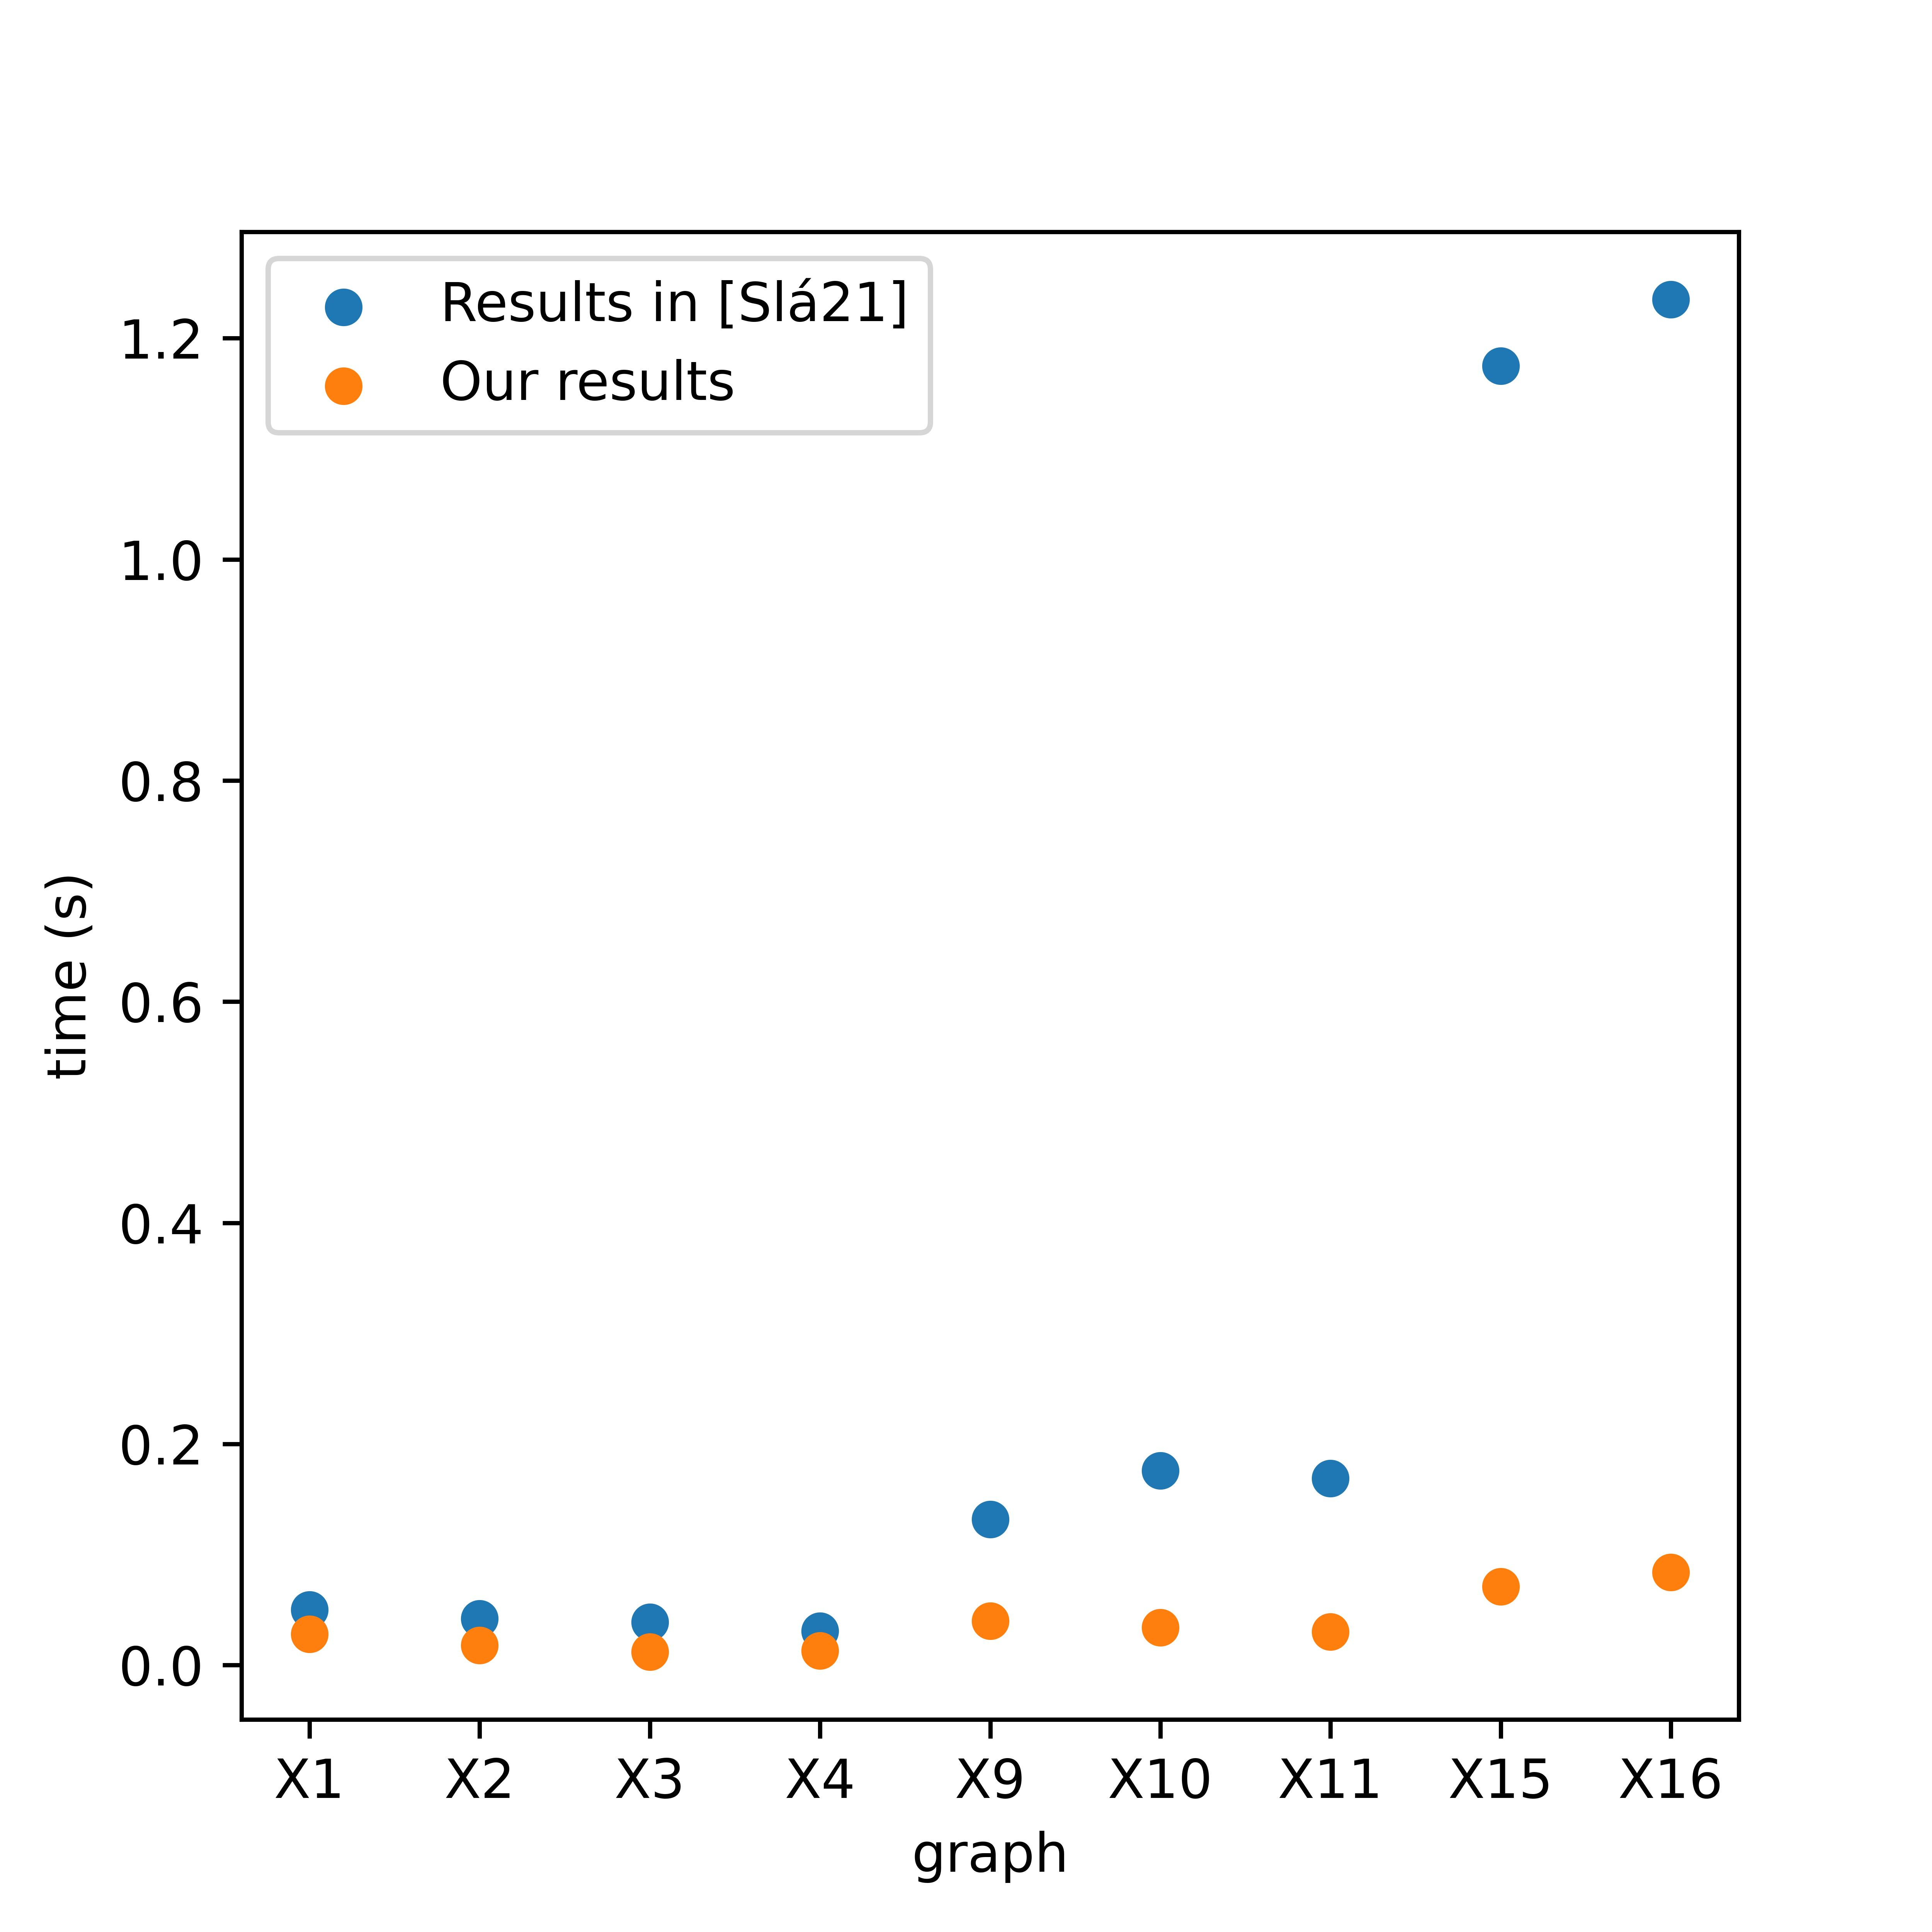
\includegraphics[scale=0.8,keepaspectratio]{images/comparison_asymmetric_slavik.jpg}
\caption{A comparison of the runtime for minimal asymmetric graphs.}
\label{fig:comparison_asymmetric}
\end{figure}

A comparison of the runtime for minimal asymmetric graphs is in Fig. \ref{fig:comparison_asymmetric}. We ran the program three times for each graph, with the times shown being averages of these runs. Our solution was marginally quicker for minimal asymmetric graphs with 6 vertices. We achieved slightly better performance for 7-vertex graphs, and the difference became more significant for 8-vertex graphs. Our solution found the partial automorphism monoid for any minimal asymmetric graph in under 0.1 seconds.

We also compared the runtimes for randomly generated graphs with 7-10 vertices with the results of these tests shown in Fig.\ref{fig:comparison_random}. Our solution achieved significantly better performance for larger graphs with 9 or 10 vertices.

\begin{figure}[H]
\centering
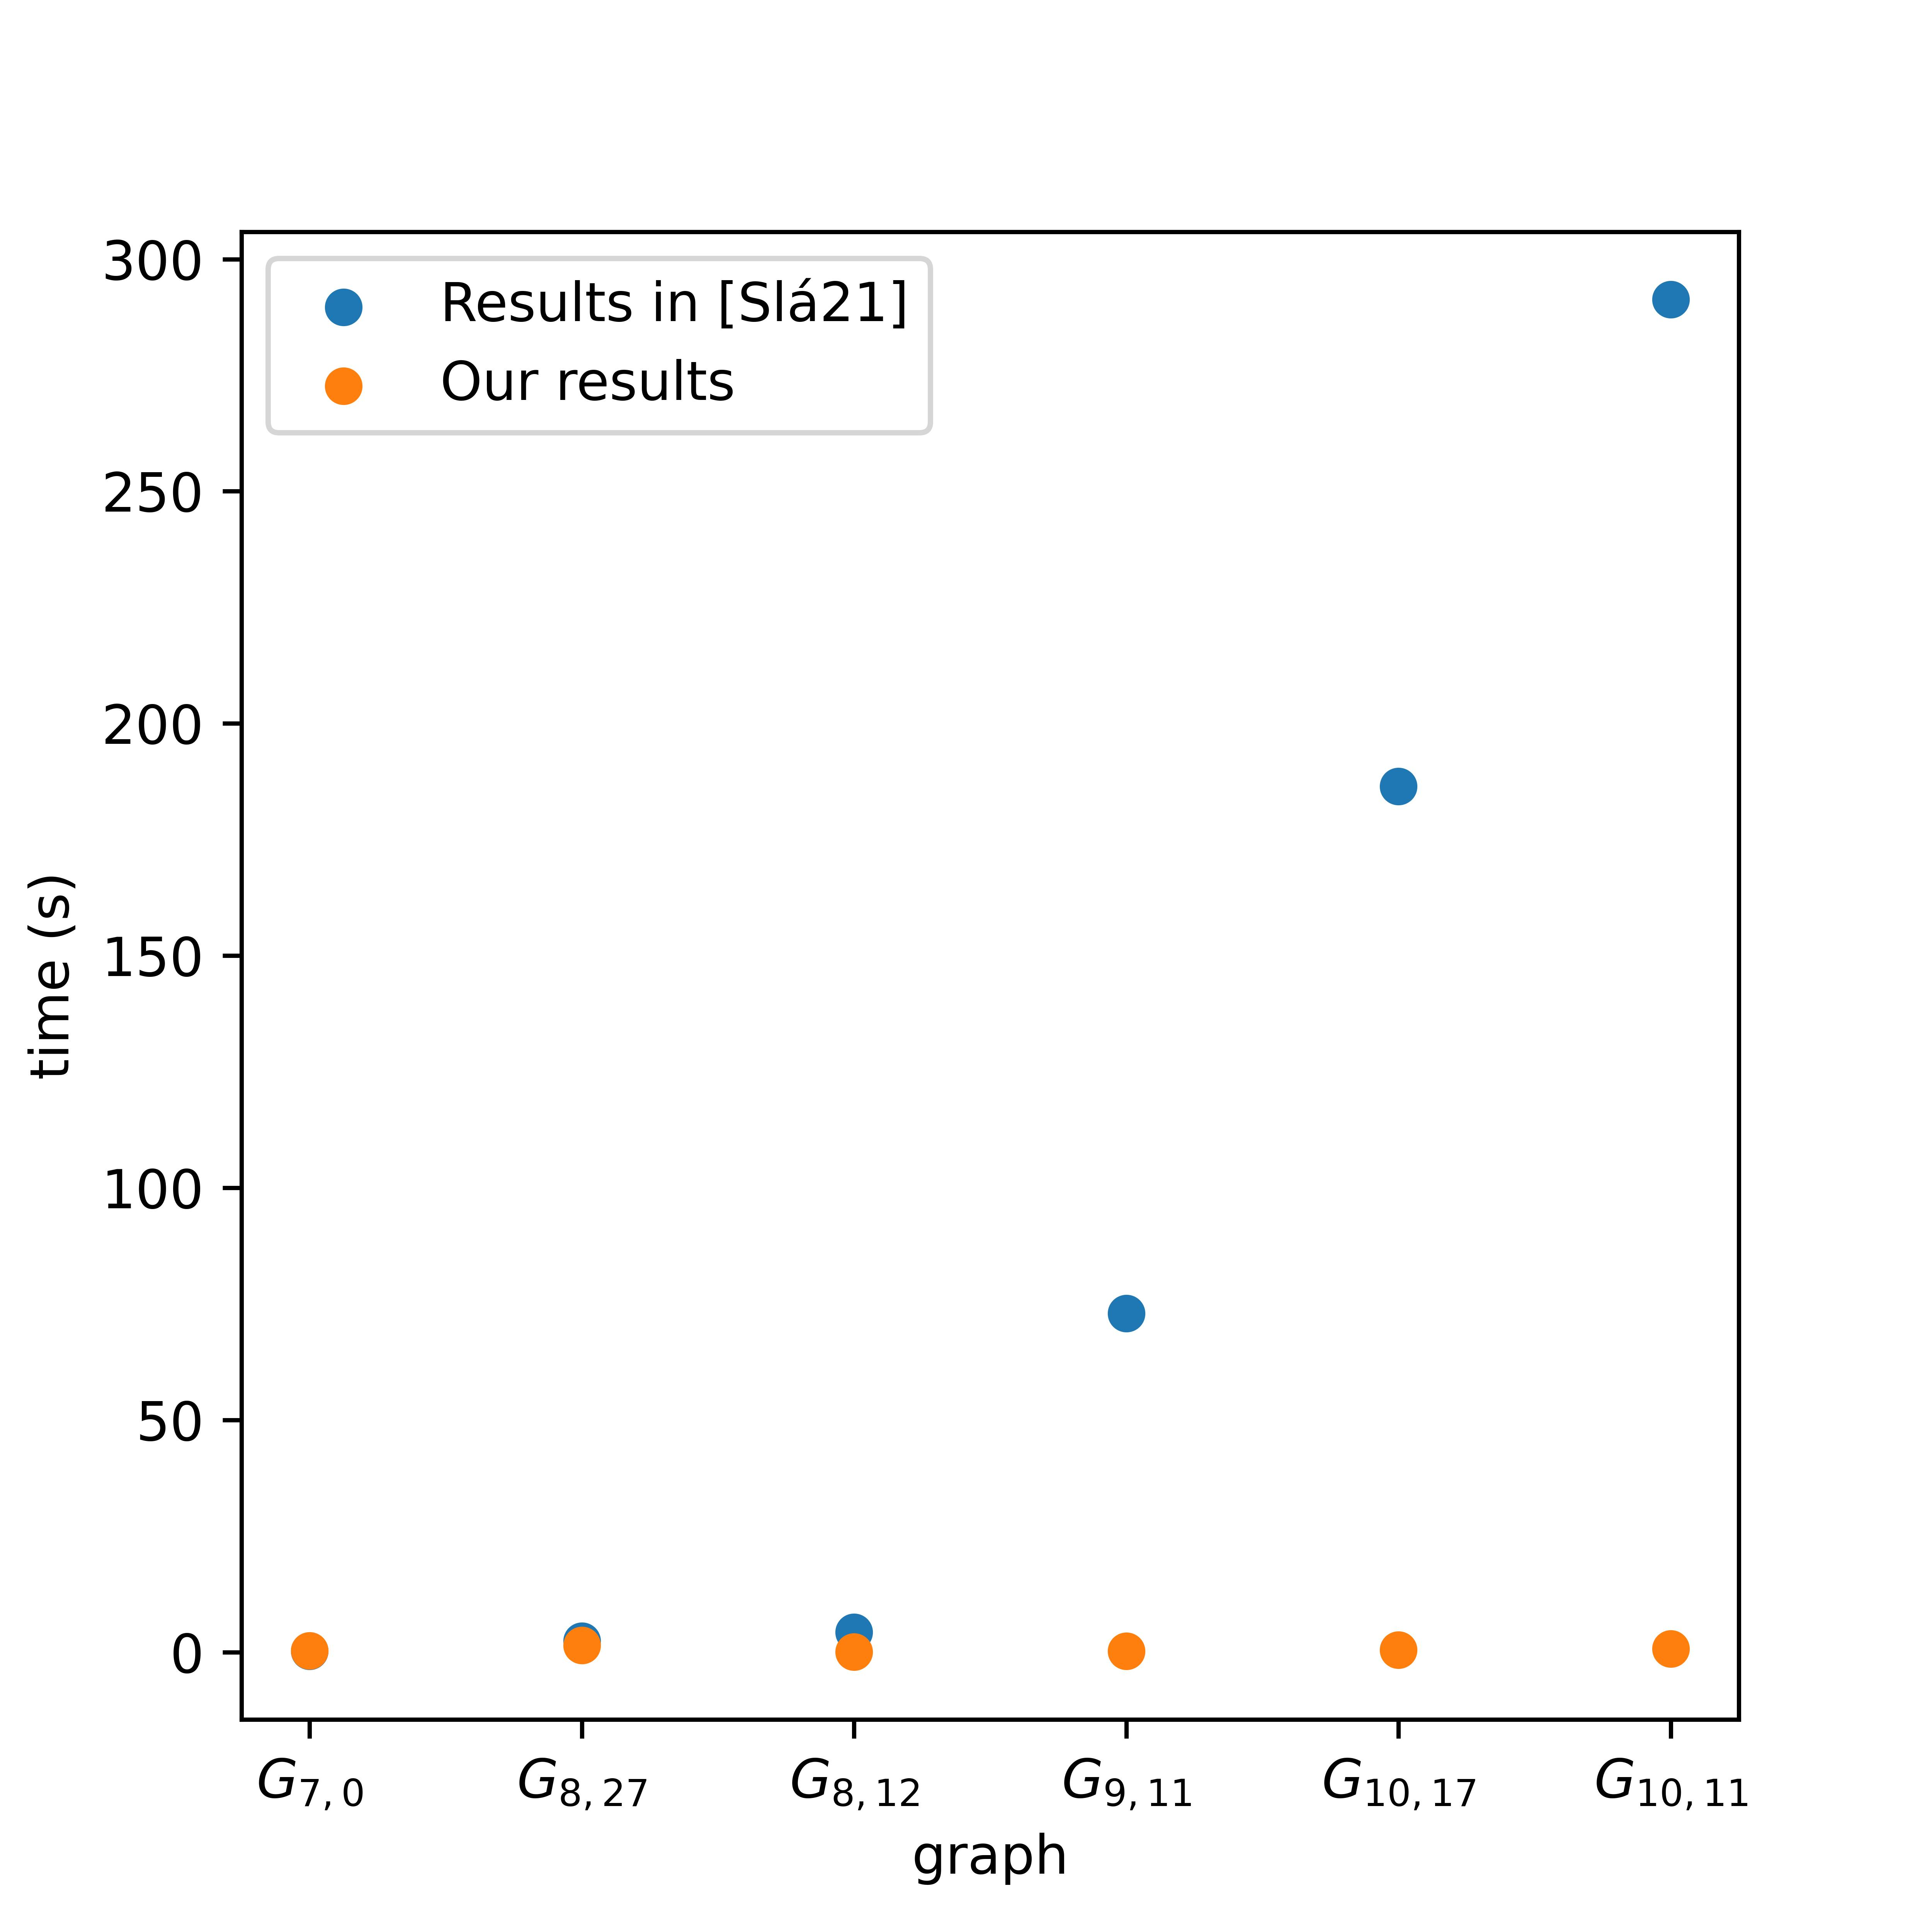
\includegraphics[scale=0.8,keepaspectratio]{images/comparison_random_slavik.jpg}
\caption{Comparison of the runtime for graphs $G_{v,e}$, where $v$ is the number of vertices and $e$ is the number of edges.}
\label{fig:comparison_random}
\end{figure}

\section{Tests on random graphs}
\label{sec:random_tests}

We ran a test involving finding all isomorphism classes, the members of each class, and constructing the partial automorphisms monoid for 151 different graphs, with 6 to 17 vertices. A vast majority of these graphs was generated randomly, with some entered manually to check for particular properties. We ran these tests using all graph filtering approaches described in \ref{sec:optimization}. We ran the test 3 times for each graph and then calculated the averages from these runs.

Let's first compare the no filtering ($nf$) approach to degree sequence filtering ($df$), with the results shown in Table \ref{tab:dfvsnf}. Degree filtering was faster for 102 graphs, and no filtering achieved better time in 49 cases. Overall, we saved around 15\% by using the $df$ approach. We see that for 10-vertex graphs, the $nf$ was around 8\% faster, but the runtime for these graphs was mostly less than 1 second with a minimal time difference between the two approaches. Generally, $nf$ achieved better performance for sparse and dense graphs ($\delta \le 0.2$ or $\delta \ge 0.8)$. In conclusion, the $df$ approach was faster on average for graphs with 12 or more vertices, with the time savings increasing for larger graphs.

\begin{table}
\begin{tabular}{ | c | c | c | c |}
\hline
\# of vertices & \# of graphs & \# times df < nf & df / nf (\%) \\
\hline
any & 151 & 102 & 85.75 \\
10 & 24 & 5 & 108.22 \\
11 & 24 & 9 & 101.96 \\
12 & 27 & 23 & 94.46 \\
13 & 28 & 25 & 80.66 \\
14 & 25 & 24 & 64.44 \\
15 & 6 & 6 &39.36 \\
16+ & 6 & 6 & 31.25 \\
\hline
\end{tabular}
\caption{\label{tab:dfvsnf} Performance comparison between degree sequence filtering ($df$) and no filtering ($nf$) approaches.}
\end{table}

\begin{table}
\begin{tabular}{ | c | c | c | c |}
\hline
\# of vertices & \# of graphs & \# times dtf < df & dtf / df (\%) \\
\hline
any & 151 & 113 & 94.47 \\
10 & 24 & 13 & 99.53 \\
11 & 24 & 18 & 97.86 \\
12 & 27 & 18 & 97.57 \\
13 & 28 & 21 & 95.77 \\
14 & 25 & 24 & 88.35 \\
15 & 6 & 6 & 87.19 \\
16+ & 6 & 6 & 69.28 \\
\hline
\end{tabular}
\caption{\label{tab:dtfvsdf} Performance comparison between degree triangle sequence filtering ($dtf$) and degree sequence filtering ($df$) approaches.}
\end{table}

Table \ref{tab:dtfvsdf} shows the comparison between the degree sequence filtering ($df$) and the degree triangle sequence filtering ($dtf$) approaches. In this case, $dtf$ achieved better performance in 113 of 151 graphs, saving 5.5\% on average. The performance of $dtf$ and $df$ was very similar for all graphs with 10 to 13 vertices, with the difference starting to be more noticeable for larger graphs with 14+ vertices.

As we already explained in Section \ref{sec:optimization} and as we can see in Table \ref{tab:dfvsnf} and Table \ref{tab:dtfvsdf}, all 3 approaches achieve relatively similar performance for graphs with less than 12 vertices. Therefore, we tried one additional approach using the following heuristic: we use the degree sequence filtering for all graphs with less than 11 vertices and for all graphs with densities $\delta \le 0.2$ or $\delta \ge 0.8$, for other graphs, we use degree triangle sequence filtering. The results of this test are in Table \ref{tab:hfvsdtf}. Using the heuristic filtering, the runtime decrease by an average of 3\% compared to the previously quickest approach, the degree triangle filtering. It was only slower on average for graphs with 10 vertices, however, the difference was negligible.

\begin{table}
\begin{tabular}{ | c | c | c | c |}
\hline
\# of vertices & \# of graphs & \# times hf < dtf & hf / dtf (\%) \\
\hline
any & 151 & 118 & 96.67 \\
10 & 24 & 8 & 102.38 \\
11 & 24 & 21 & 94.14 \\
12 & 27 & 24 & 95.11 \\
13 & 28 & 25 & 95.76 \\
14 & 25 & 21 & 94.51 \\
15 & 6 & 6 & 93.62 \\
16+ & 6 & 4 & 96.14 \\
\hline
\end{tabular}
\caption{\label{tab:hfvsdtf} Performance comparison between degree triangle filtering ($dtf$) and heuristic filtering ($hf$) approaches.}
\end{table}

\section{Asymmetric depth}

Especially for larger graphs, it might be useful to study the structure of the graph to predict the number of partial symmetries the graph has. We introduce a definition for \emph{asymmetric depth}, a metric that can measure the asymmetricity of graphs.

\begin{definition}
\label{def:asymmetric_depth}
For any $n$ vertex graph, asymmetricity level $AsymL = i$ means all $n, n-1, n-2, \cdots, n - i$ vertex-induced subgraphs are asymmetric and pairwise non-isomorphic.

The asymmetric depth of a graph G is a number $i$, such that G has an asymmetricity level $i$, but not $i+1$. We use $AsymD(G)$ to denote the asymmetric depth of graph G.
\end{definition}

For example, when given two graphs with the same number of vertices, one can make the assumption the graph with higher asymmetric depth will have fewer partial symmetries than the other graph.

We created our application to provide an interface for easy work with graphs, graph symmetries, and partial symmetries. As a result, it allowed us to create a simple script to answer the following question:

\emph{Does any asymmetric graph with $n, n \le 10$ vertices exist with $AsymL = 1$?}

We used the collection of all unlabelled simple graphs generated by McKay and published in GAP format \cite{mckaycol}. We know there are no asymmetric graphs with $2 \leq n \leq 5$ vertices \cite{er63}. Since there are no asymmetric graphs with 5 vertices, we know that none of the 8 asymmetric graphs with 6 vertices, of which all are minimal, have asymmetric subgraphs with 5 vertices\cite{oeisasym}\cite{sch17}.

We then checked all 1044 graphs with 7 vertices, of which 152 are asymmetric \cite{oeisgraphs}. We found that none of these graphs have $AsymL = 1$.

We then found that of the 3696 asymmetric unlabelled graphs with 8 vertices, there are 8 graphs with asymmetricity level 1. We also checked all asymmetric graphs with 9 and 10 vertices and found 2608 such 9-vertex graphs and more than a million 10-vertex graphs with asymmetricity level 1.

Based on the findings from \cite{er63}, we know that "almost all finite graphs are asymmetric". The number of asymmetric graphs with $n$ vertices gets closer to the total number of possible graphs with $n$ unlabeled vertices as $n$ grows. We also expect the number of asymmetric graphs with $n$ vertices with asymmetricity level 1 to increase as $n$ grows. We can see this in our experiments, as we found 8 8-vertex graphs with asymmetricity level 1, from a total of 3696 8-vertex asymmetric graphs. For $n=9$ there are 135004 asymmetric graphs, of those 2608 have asymmetricity level 1, and for $n=10$ there are more than a million graphs with asymmetricity level 1 of almost 8 million asymmetric graphs.
\vspace{0.5cm}

We then extended our original question:

\emph{Are there graphs with asymmetricity level 2?}

We checked all previously found graphs and discovered no such graphs among graphs with 10 or fewer vertices. We did not check all unlabelled graphs with 11 vertices, since there are more than a billion such graphs. Instead, we changed our approach. We took an asymmetric graph with 10 vertices and created all possible 11-vertex graphs by adding a new vertex to it. In total, there are $2^{10}$ possible ways of adding a new vertex to a 10-vertex graph. Using this approach, we found 11-vertex graphs with asymmetricity level 2.

We assume the reason why there are such graphs with 11 vertices but not with 10 vertices is that for a graph with 10 vertices, there are $\binom{10}{8}$ = 45 induced subgraphs with 8 vertices, but there are only a total of 3696 8-vertex asymmetric graphs, but for 11 vertex graph there are $\binom{11}{9}$ = 55 9-vertex induced subgraphs, but a total of 135004 9-vertex asymmetric graphs.

Since we were able to answer our previous question, we proposed the following tasks:

\begin{enumerate}
\item \emph{For any given graph $G$, find $AsymD(G)$.} \label{item:q1}
\item \emph{Find an $n$-vertex graph with asymmetricity level $i$.} \label{item:q2}
\item \emph{Find the maximal asymmetric depth any $n$-vertex graph can have.} \label{item:q3}
\end{enumerate}

Utilizing the previous findings and our extensive library, we quickly answered task \ref{item:q1} by implementing a function $find\_asym\_d$, which takes a graph as an argument and returns its asymmetric depth.

For task \ref{item:q2}, we extended the approach described previously. By taking any $n$-vertex asymmetric graph, we can create a $n+1$-vertex graph by adding a new vertex. In total, there are $2^n$ different ways of doing this, since the new vertex is either isolated or we add it as a neighbor to any $k, 1 \leq k \leq n$-vertex subset of the set of vertices. We then use the function $has\_asymmetricity\_level$ to verify if the new graph has asymmetricity level $i$. Using this approach, we found graphs with 14 vertices and asymmetricity level 3. However, this approach is computationally difficult and would not be appropriate for finding all $n$ vertex graphs with a given asymmetricity level.

Clearly, for a graph with $n$ vertices, there is no point in checking if it has asymmetricity level $i$ if $\binom{n}{i} > Asym(i)$, where $Asym(i)$ is the total number of asymmetric graphs with $i$ vertices. For example, for 11 vertex graphs and asymmetricity level 4, we have $\binom{11}{7}$ = 330 vertex-induced subgraphs, yet only 152 asymmetric 7-vertex graphs exist.

Finally, we wanted to find graphs with an asymmetric depth of 4 or more. We randomly generated 15-30 vertex graphs, calculated their asymmetric depth, and were able to find graphs with asymmetric depth 4.

Due to the combinatorial explosion occurring when working with graphs, their subgraphs, and symmetries, answering tasks \ref{item:q2} and \ref{item:q3} is a computationally difficult problem. We believe the initial findings presented here can serve as a baseline for future research in this area.

\section{Number of partial automorphisms}

Due to how quickly the number of partial symmetries rises when the number of vertices increases, we wanted to know if we can predict the number of partial symmetries of a graph by looking at its structure. For this reason, we calculated the number of partial symmetries for all unlabelled graphs with $n, 3 \leq n \leq 9$ vertices.

To find the number of partial automorphisms of a given graph, it is only necessary to find all isomorphism classes and all their members. We can calculate the number of partial symmetries of an isomorphism class $I$ using the formula $|I|^2 \times |Aut(rep_I)|$, where $rep$ acts as a representative of $I$.

\begin{figure}[H]
\centering
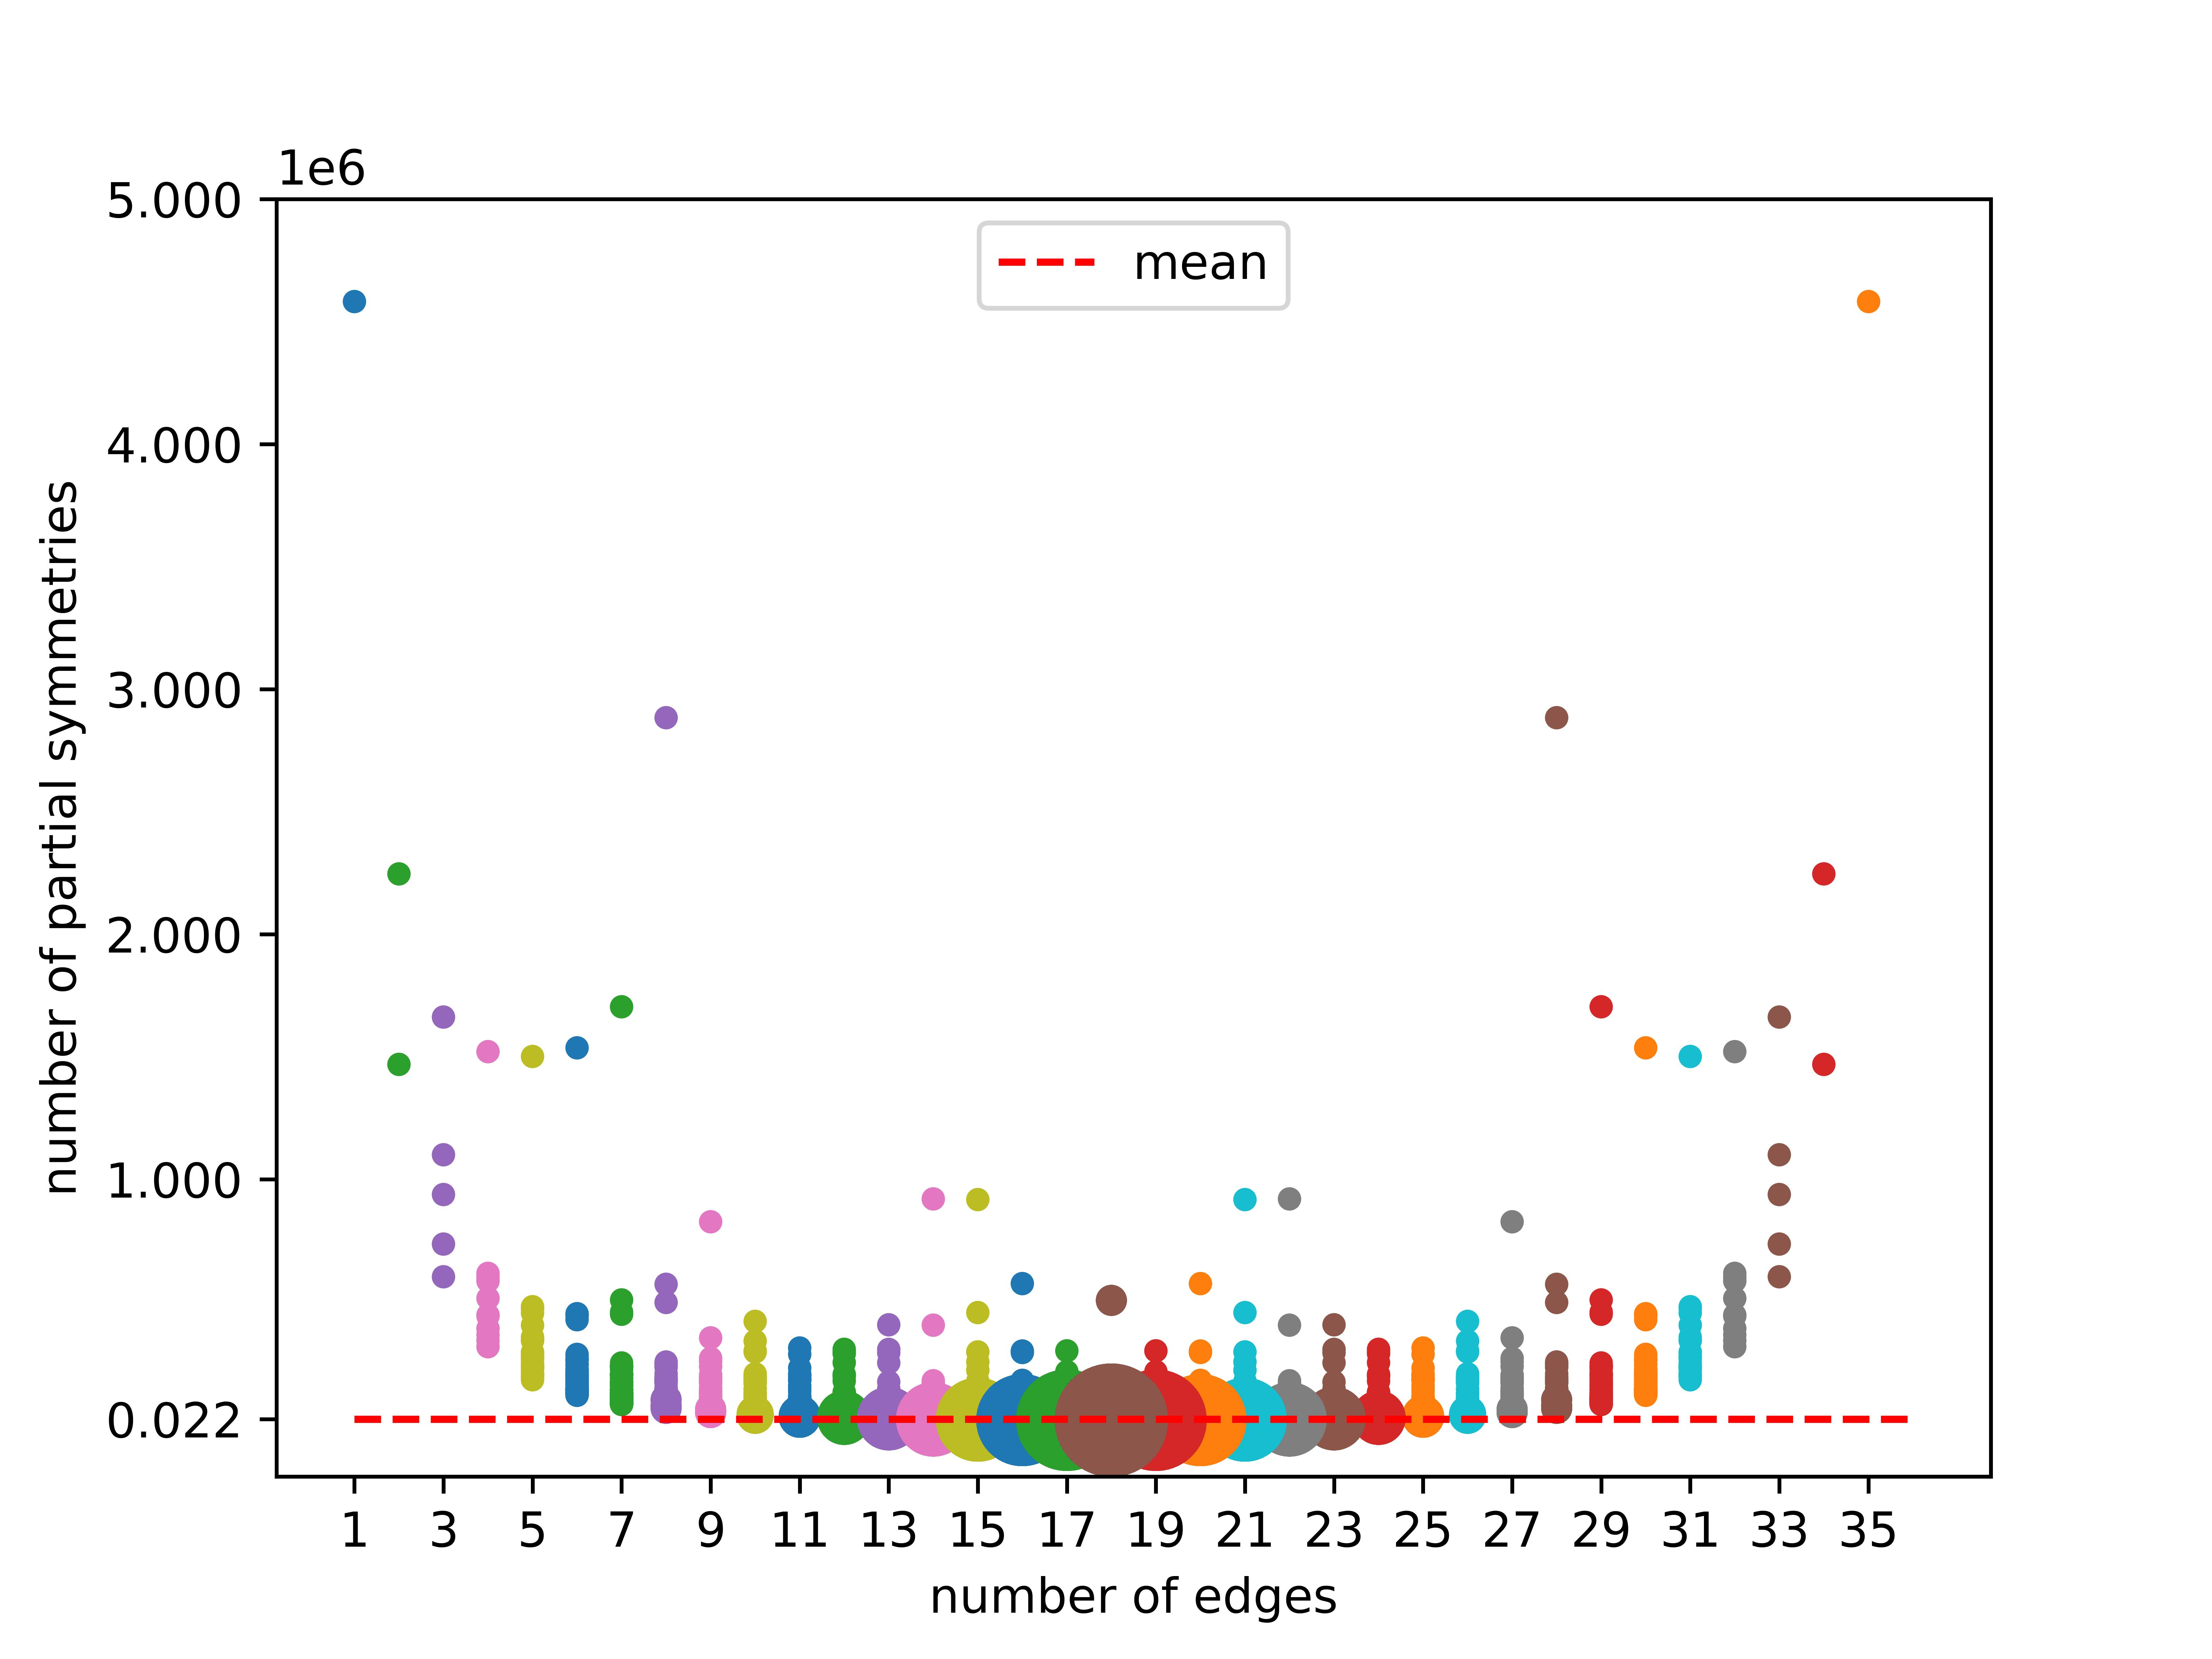
\includegraphics[scale=0.8,keepaspectratio]{images/9_vertices_minus_complete.jpg}
\caption{The number of partial symmetries for all 9-vertex graphs, dot size denotes the number of graphs.}
\label{fig:partial9}
\end{figure}

Fig. \ref{fig:partial9} shows the number of partial symmetries for graphs with 9 vertices, where we excluded $K_9$ and its complement. The size of the dot scales proportionally to the number of graphs having that number of partial symmetries. One can quickly notice how symmetrical this image is. It is to be expected since we know that a graph and its complement share the same partial automorphism monoid structure and therefore have the same number of partial symmetries.

\begin{figure}[H]
\centering
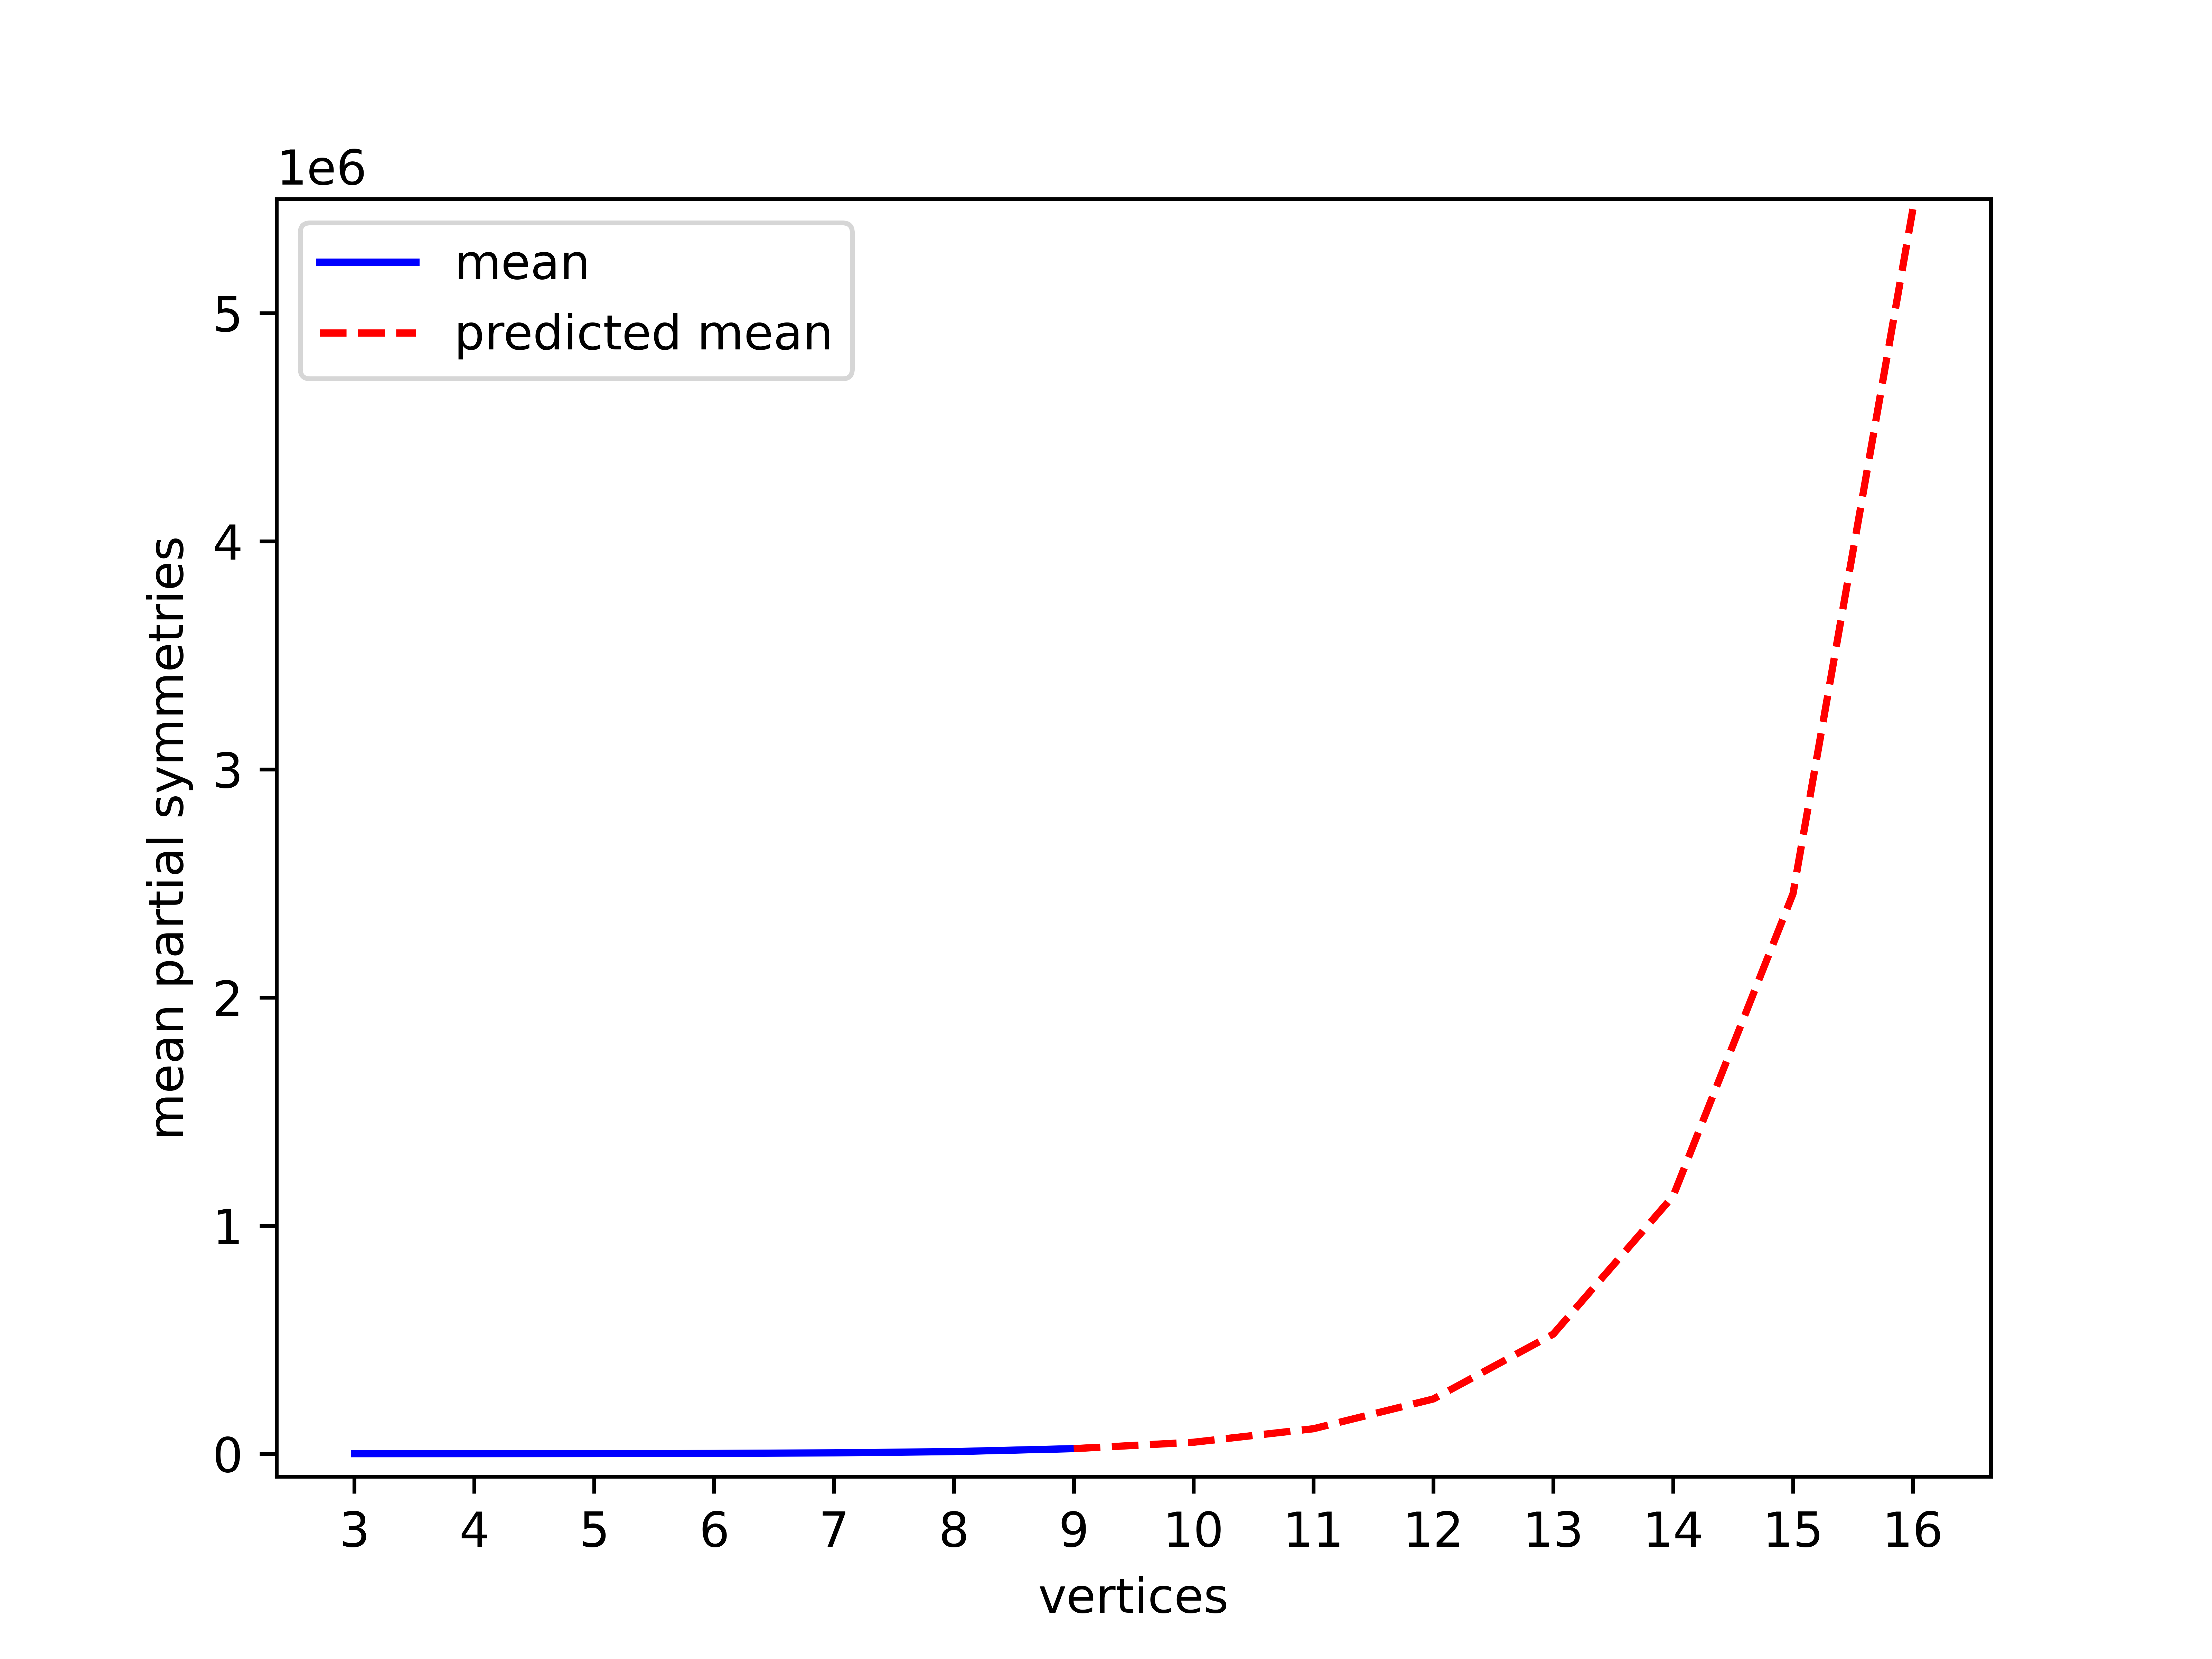
\includegraphics[scale=0.8,keepaspectratio]{images/mean_values_prediction.png}
\caption{Mean number of partial symmetries for graphs with 3-9 vertices with predictions for graphs with 10-16 vertices.}
\label{fig:prediction}
\end{figure}

We made the following observations by studying the results obtained for all graphs with 9 or fewer vertices. Firstly, for any $n$-vertex graph, the number of partial symmetries is equal to the number of partial permutations of an $n$-set in two cases: for the complete graph $K_n$ and its complement (graph with $n$ vertices and 0 edges) \cite{partialperm}. Removal of just one edge from $K_n$ significantly reduces the number of partial symmetries. For $n = 9$, we go from 17572114 partial symmetries for $K_9$ to 4582270 partial symmetries for $K_9 \setminus \{e\}$.

Next, we notice that for graphs with $k$ edges, $1 \leq k \leq 9$, there is always one graph with a number of partial symmetries higher than other $k$-edge graphs. These graphs consist of a $k$-vertex star with all other vertices being isolated.

Despite $K_9$ having more than 4.5 million partial symmetries, the mean number of partial symmetries for 9 vertex graphs is only 22154, a decrease of 99.5\%. We also calculated the mean values for graphs with 3 to 8 vertices, and based on the data, we predicted the mean of partial symmetries for graphs with less than 17 vertices. The prediction can be seen in Fig. \ref{fig:prediction}.